%WMS
%Kelompok 3 D4 TI-3D
%Aditya Pratama Dharma-1154043
%Andi Syahjaratu Daur-1154092
%Bendra Wardana-1154015
%Dini Islamiani Lestari-1154039
%Nur Rahmawati-115124

\section{Deskripsi WMS}
  Web Map Service adalah salah satu jenis penggambarakn OGC Layanan model layanan web dan ia menyediakan platfrom
multi-interoperability.Karya ini menghadirkan sebuah metode untuk menerapkan layanan peta web OGC berdasarkan teknik
Layanan Web dan memperkenalkan proses terperinci.
  
    Web Map Service (wms) memberikan informasi kepada pengguna internet oleh tata ruang peta gambar.Umumnya,yang tersimpan
di dalam tata ruang data tersebut data vektor itu adalah panjang untuk menciptakan data vektor peta gambar.
setiap sub-rectangle dikirim ke sebuah wmssub-maps node untuk menghasilkan sekumpulan peta yang dihasilkan merekontruksi
dengan semuanya sub-maps.Semua sub-maps dihasilkan di paralel,jadi makin sedikit waktu seluruh yang habis memproduksi
sebuah peta.

   Web Map Service (WMS) memberikan informasi kepada pengguna internet oleh tata ruang peta gambar.Umumnya,
yang tersimpan di dalam tata ruang data tersebut data vektor .Itu adalah panjang ayub untuk 
menciptakan data vektor peta gambar dari .Biaya untuk mengurangi waktu , maka kami memanfaatkan linux cluster .
Ketika peta diminta, itu adalah suatu koordinat lingkup didefinisikan dengan xmin persegi panjang,ymin,xmax, 
ymax harus dispesifikasikan .Kami merancang beban keseimbangan menurut algoritma untuk membagi permintaan ke dalam 
beberapa sub-rectangles .

   Setiap sub-rectangle dikirim ke sebuah wms sub-maps node untuk menghasilkan sekumpulan .
Peta yang dihasilkan akan merekonstruksi dengan semuanya ini sub-maps .Semua ini sub-maps dihasilkan di paralel, 
jadi makin sedikit waktu yang seluruh habis di memproduksi sebuah peta .Bagaimana untuk membagi menurut adalah 
kunci masalah permintaan .Pertama , kami menghadirkan metode untuk menghitung tingkat 2d bobot beban distribusi peta lingkup .
Kedua , node beban kemampuan yang dievaluasi .Kemudian , penulis hadirmetode menurut untuk membelah seluruh.
Kertas ini juga membahas algoritma kinerja pelaksanaan .

\subsection{Pengenalan peta map service}
   Pengenalan Peta map Service (WM)s menghasilkan peta secara spasial direferensikan data dari informasi geografis secara dinamis. 
Standar internasional ini mendefinisikan sebuah "peta" untuk menjadi penggambaran tentang informasi geografis 
sebagai file gambar digital cocok untuk ditampilkan pada layar komputer. Peta tidak data itu sendiri. 
Wms-dihasilkan maps umumnya diterjemahkan dalam format bergambar seperti PNG,GIF atau JPEG,atau kadang-kadang sebagai
elemen-elemen grafis berbasis vektor dalam Scalable Vector Grafis (SVG) atau Komputer Web Metafile Grafis (WebCGM format).

   WMS pelaksanaannya dengan Membuka Geospatial Konsorsium Peta Web Service (WMS menentukan spesifikasi) untuk gridded multidimensi data lingkungan. WMS dapat membaca data dalam jumlah besar format data ilmiah umum - khususnya format NetCDF dengan perubahan iklim dan konvensi Perkiraan kemudian efisien menghasilkan gambar peta di ribuan mengkoordinir sistem referensi. Ia dirancang untuk memerlukan konfigurasi minimal dari administrator sistem pada saat digunakan dengan alat bantu klien yang sesuai, menyediakan pengguna akhir dengan cara interaktif untuk memvisualisasikan data tanpa perlu mendownload file besar atau menafsirkan meta data kompleks. 

Data WMS biasanya digunakan untuk membandingkan data yang sudah kita buat dengan data yang dibuat oleh pihak lain, atau juga sering kali
digunakan sebagai pelengkap dalam pembuatan peta.

\subsection{Interoperability antara WM dan grid data lingkungan}

Dalam WMS, unit penting informasi merupakan lapisan. Setiap lapisan dapat ditampilkan dalam jumlah Gaya, setiap dikaitkan dengan sebuah
legenda. Lapisan mungkin yang dapat ditampilkan atau non-yang dapat ditampilkan dan bisa diatur hierarchically. Tiga operasi utama dapat
dilakukan oleh klien WM menentukan standar: Permintaan GetCapabilities dokumen XML berisi metadata tersedia pada lapisan dan kemampuan
layanan lain; permintaan GetMap gambar peta animasi atau sesuai dengan pilihan pengguna Layer, Style, sejauh geografis dan resolusi dan
permintaan GetFeatureInfo informasi lebih lanjut tentang lokasi geografis tertentu, yang diwakili oleh piksel tertentu dalam gambar
peta.

Disini menjelaskan ncWMS, sebuah implementasi dari spesifikasi Web Map Service (WMS) geospasial untuk data lingkungan gridded
multidimensional. ncWMS dapat membaca data dalam sejumlah besar format data ilmiah - terutama format CDS Bersih dengan konvensi iklim 
dan perkiraan - kemudian secara efisien menghasilkan citra peta dalam ribuan sistem referensi koordinat yang berbeda.

Tujuan ncWMS ia adalah untuk dapat menghasilkan beberapa jenis visualisasi berbeda (maps, transects bagian vertikal, dsb.) secara
efisien data dari diselenggarakan dalam format file yang berbeda dan mengkoordinir sistem referensi (CRSs).
\begin{figure}[ht]
\centerline{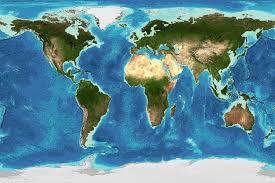
\includegraphics[width=1\textwidth]{figures/wmsimage.jpg}}
\caption{Menjeleskan tentang Interoperability antara WMS dan grid data lingkungan}	
\label{Web Map Service}
\end{figure}
pada gambar \ref{wmsimage.jpg} dijelaskan bahwa interoperability antara WMS dan Grid Data Lingkungan.

\section{mengimplementasikan NcWMS sebagai aplikasi Web Java}
NcWMS diimplementasikan sebagai aplikasi web Java, dikemas sebagai arsip web (WAR) untuk file yang standar penempatan wadah servlet
seperti Apache Tomcat. Java telah dipilih sebagai bahasa menerapkan karena banyak penyedia data lingkungan sudah menggunakan teknologi
server-side Java dan karena ketersediaan berkualitas tinggi dan perpustakaan yang kuat seperti Java-NetCDF.

Banyak WMS client, termasuk Godiva2 client yang dibundel dengan ncWMS, adalah tidak hanya berasal dari client yang membuat permintaan
GetMap menggunakan nomor yang terbatas dari kotak pengikat yang telah diperbaiki. Hal ini akan meningkatkan skalabilitas dari sistem
secara keseluruhan dengan mengizinkan permintaan diulangi untuk gambar yang sama untuk dilayani dari cache level-aplikasi. Karena itu
ncWMS menerapkan cache seperti (lihat diagram arsitektur dalam pohon ara.  Catatan bahwa cache ini berpendapat array data, tidak gambar
akhir: ini memungkinkan pengguna untuk mengubah parameter penata dari suatu gambar (misalnya Palet deep warna) tanpa re-ekstrak data
dari file sumber, mempercepat visualisasi interaktif. Banyak administrator sistem memilih juga untuk menerapkan cache ubin di atas
ncWMS, yang lebih jauh dapat meningkatkan performa dan skalabilitas.

ncwms biasanya menyajikan data spasial peta atau citra, yang akan menjadi layer saat visualisasi di browser.
biasanya dengan melakukan request getmap, Getmap merupakan salah satu operasi wms, akan dihasilkan tampilan peta berupa layer yang
melapisi (overlay) peta pada dasar google maps. peta yang berferensi geografis dihasilkan dari sebuah web map service, dan peta ini
biasanya disajikan dalam format gambar seperi PNG, GIF dll.

\subsection{Menjelaskan tentang layanan WMS}
Layanan web map service  meningkatkan dengan  adanya fisheye pandangan metode untuk cartographic data .Sementara banyak studi difokuskan
pada pandangan fisheye,masalah yang banyak besar distorsi yang memetakan mereka semuanya memiliki lebih dari wilayah dan / atau high
density jalan di perbatasan peta belum diatasi .Untuk sepenuhnya menghapus distorsi di kedua fokus dan konteks daerah.

\section{Beberapa operasi wms pada tahap implementasi}
WMS memiliki tiga buah operasi wms pada saat tahap implementasi yaitu : GetCapabilities merupakan deskripsi informasi yang dimiliki wms
dan parameter perimintaan yang dapat diterima, Getmap yaitu peta dengan paramametrer dimensi, Getfeaure info yaitu meminta informasi 
mengenai fitur tertentu yang ditampilkan pada peta,Web Map Service (WMS) memberikan informasi kepada pengguna internet oleh tata ruang peta gambar.

\subsection{WMS}
WMS (Web Map Services) tidak hanya dapat menghasilkan gambar raster tetapi juga gambar vektor. Contohnya  adalah SVGT (Scalable Vector
Graphics Tiny) yang merupakan bagian dari SVG (Scalable Vector Graphics) yang digunakan pada piranti mobile device. Mahalnya biaya
komunikasi antara handheld device dengan jaringan internet melalui GPRS (Global Pocket Radio System) menimbulkan sebuah masalah dalam
penerapan aplikasi mobile mapping. Untuk mengeliminasi masalah tersebut, harus dibuat sebuah aplikasi mobile mapping yang dapat mentransfer data sekecil mungkin.

Dengan bantuan teknologi web map service  sejumlah besar layanan wms dikembangkan dan dirilis ke network. tidak untuk organik di antara
peta layanan web, menggunakan sangat kesulitan mendapatkan dan memanfaatkan ini services. satu jenis layanan web peta mesin pencari
frame yang diajukan, termasuk url mesin pencari, kemampuan basis data dan kemampuan dokumen respon analyzer.Web map service merupakan suatu komponen software yang merupakan suatu komponen software yang merupakan self-containing.wms yang paling banyak  diadopsi dan populer yang digunakan peta web service (WMS),spesifikasi yang menguraikan sebuah mekanisme komunikasi memungkinkan menguraikan produk perangkat lunak untuk meminta dan memberikan peta preassembled citra dikompile gambar peta, yang mungkin berisi kedua kordinat dan data raster yang meminta klien




  
  
